%% Standalone source of one report figure. Rebuild: pdflatex -output-directory=.. fig-02-thirteen-steps.tex
\documentclass[11pt]{standalone}
\usepackage[T1]{fontenc}
\usepackage[utf8]{inputenc}
\usepackage{lmodern}
\usepackage{microtype}
\usepackage{amsmath,amssymb}
\usepackage{xcolor}
\usepackage{tikz}
\usetikzlibrary{arrows.meta,positioning,shapes.geometric,fit,calc,backgrounds}
\usepackage{pgfplots}
\usepackage{pgfplotstable}
\pgfplotsset{compat=1.18}
\setlength{\textwidth}{472.31595pt}  %% = the report's text width, so widths given in \textwidth match
\definecolor{gmblue}{HTML}{0B3D6E}
\definecolor{gmok}{HTML}{1E7B34}
\definecolor{gmwarn}{HTML}{B35C00}
\definecolor{gmbad}{HTML}{A32020}
\definecolor{gmgrey}{HTML}{5A5F66}
\definecolor{gmlight}{HTML}{EEF3F8}
\definecolor{gmteal}{HTML}{1B7A8C}
\newcommand{\done}{\textcolor{gmok}{\textbf{Done}}}
\newcommand{\partly}{\textcolor{gmwarn}{\textbf{Partly}}}
\newcommand{\pending}{\textcolor{gmbad}{\textbf{Pending}}}
\newcommand{\pass}{\textcolor{gmok}{\textbf{PASS}}}
\newcommand{\fail}{\textcolor{gmbad}{\textbf{FAIL}}}
\newcommand{\code}[1]{\texttt{\small #1}}
\newcommand{\INR}{INR~}
\newcommand{\gbar}[5]{\fill[#5] (#1,-#3+0.32) rectangle (#2,-#3-0.32);
  \node[anchor=east,font=\scriptsize] at (-0.3,-#3) {#4};}

\tikzset{
  box/.style={draw=gmblue, rounded corners=3pt, fill=gmlight, align=center, font=\small, inner sep=5pt,
              minimum height=9mm},
  gstep/.style={draw=gmblue, rounded corners=3pt, fill=white, align=center, font=\footnotesize, inner sep=4pt,
               text width=27mm, minimum height=11mm},
  st/.style={draw=gmblue, rounded corners=6pt, fill=gmlight, font=\scriptsize\ttfamily, inner sep=3pt,
             minimum height=6mm},
  arr/.style={-{Stealth[length=2.2mm]}, thick, gmblue},
  darr/.style={-{Stealth[length=2mm]}, gmgrey, dashed},
}

\begin{document}
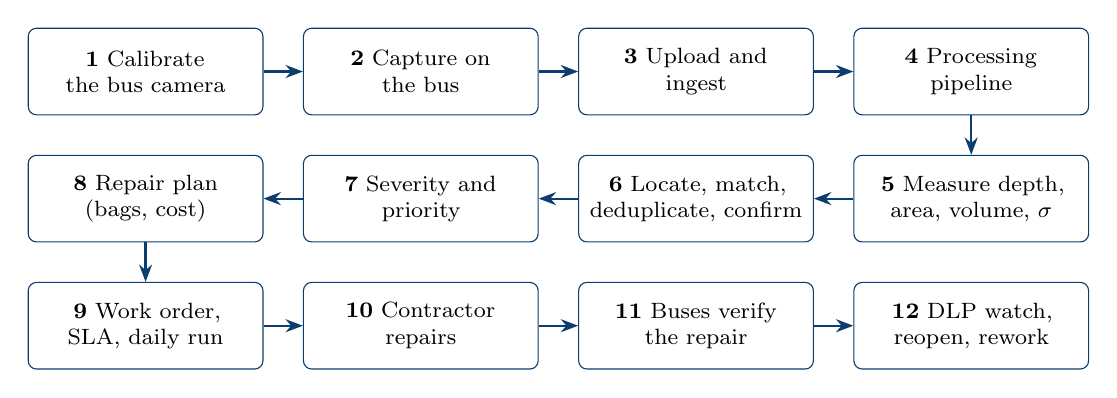
\begin{tikzpicture}[node distance=5mm and 5mm]
  \node[gstep] (s1) {\textbf{1} Calibrate\\the bus camera};
  \node[gstep, right=of s1] (s2) {\textbf{2} Capture on\\the bus};
  \node[gstep, right=of s2] (s3) {\textbf{3} Upload and\\ingest};
  \node[gstep, right=of s3] (s4) {\textbf{4} Processing\\pipeline};
  \node[gstep, below=of s4] (s5) {\textbf{5} Measure depth,\\area, volume, $\sigma$};
  \node[gstep, left=of s5] (s6) {\textbf{6} Locate, match,\\deduplicate, confirm};
  \node[gstep, left=of s6] (s7) {\textbf{7} Severity and\\priority};
  \node[gstep, left=of s7] (s8) {\textbf{8} Repair plan\\(bags, cost)};
  \node[gstep, below=of s8] (s9) {\textbf{9} Work order,\\SLA, daily run};
  \node[gstep, right=of s9] (s10) {\textbf{10} Contractor\\repairs};
  \node[gstep, right=of s10] (s11) {\textbf{11} Buses verify\\the repair};
  \node[gstep, right=of s11] (s12) {\textbf{12} DLP watch,\\reopen, rework};
  \draw[arr] (s1)--(s2); \draw[arr] (s2)--(s3); \draw[arr] (s3)--(s4); \draw[arr] (s4)--(s5);
  \draw[arr] (s5)--(s6); \draw[arr] (s6)--(s7); \draw[arr] (s7)--(s8); \draw[arr] (s8)--(s9);
  \draw[arr] (s9)--(s10); \draw[arr] (s10)--(s11); \draw[arr] (s11)--(s12);
\end{tikzpicture}
\end{document}
